% Section content template for individual Educative lessons
% This file contains the actual content for a specific section
% Generated from Educative API section content

% Section: Sequence Diagram for the Car Rental System
% Section ID: 6250981438521344
% Section Slug: sequence-diagram-for-the-car-rental-system
% Generated: 2025-12-12T14:51:47.446424

Sequence diagrams illustrate the flow of messages and method calls between various actors and objects in the system as they participate in a business process. They are invaluable for visualizing how objects collaborate to complete key scenarios.
\\
In this lesson, we will create sequence diagrams for two essential interactions in the car rental system:

\begin{itemize}
\item
\protect\phantomsection\label{jQbYjt592pl8TSK3WjCAj}
Vehicle reservation (the customer reserves a vehicle)
\item
\protect\phantomsection\label{pSp67cyccj959k-oyTTNK}
Reservation cancellation (the customer cancels a reservation)
\end{itemize}

\subsection{Vehicle reservation}\label{sqMKRH7fvLTFXNz_Ko22T}
\\
The sequence diagram for vehicle reservation should have the following actors and objects that will interact with each other:
\\
\textbf{Actors and objects involved:}

\begin{itemize}
\item
\protect\phantomsection\label{FoC2UbwwwRlInM9pFW8FW}
\textbf{Actor:} \texttt{Customer} (or \texttt{Receptionist}, acting on behalf of a customer)
\item
\protect\phantomsection\label{-uQJ03e4is6RUiazkGUpl}
\textbf{Objects:} \texttt{VehicleCatalog}, \texttt{CarRentalSystem}, \texttt{VehicleReservation}, \texttt{Payment}, and \texttt{Notification}
\end{itemize}

\subsubsection{Interaction steps}\label{qD9qzfmW4leD1MqsBw3tN}

\begin{enumerate}
\item
\protect\phantomsection\label{4SMn5fxy9pio37RnYAMDf}
\textbf{Search for vehicle:}

\begin{enumerate}
\item
\texttt{Customer} requests to search available vehicles.
\item
\texttt{CarRentalSystem} interacts with the \texttt{VehicleCatalog} to retrieve available vehicles.
\item
\texttt{VehicleCatalog} returns a list of available vehicles.
\end{enumerate}
\item
\protect\phantomsection\label{jUyslL1Hd3VTbJZTGtQ8U}
\textbf{Select and reserve vehicle:}

\begin{enumerate}
\item
\texttt{Customer} selects a vehicle to reserve.
\item
\texttt{CarRentalSystem} checks if the vehicle is available.
\item
If available, the \texttt{CarRentalSystem} creates a new \texttt{VehicleReservation} object.
\end{enumerate}
\item
\protect\phantomsection\label{ThQyx33nc3n4kd6ZFpsCW}
\textbf{Payment processing:}

\begin{enumerate}
\item
\texttt{CarRentalSystem} calculates the reservation fee.
\item
\texttt{CarRentalSystem} prompts the \texttt{Customer} for payment.
\item
\texttt{Customer} initiates the payment (via \texttt{Payment} object).
\item
\texttt{Payment} is processed.

\begin{enumerate}
\item
\textbf{If successful:}

\begin{enumerate}
\item
\texttt{CarRentalSystem} updates the reservation status to ``confirmed.''
\item
\texttt{CarRentalSystem} triggers a \texttt{Notification} to the customer (reservation confirmation).
\item
\texttt{Customer} receives confirmation that the reservation is successful.
\end{enumerate}
\item
\textbf{If unsuccessful:}

\begin{enumerate}
\item
\texttt{CarRentalSystem} deletes/cancels the reservation.
\item
\texttt{CarRentalSystem} triggers a \texttt{Notification} to the customer (reservation failed).
\item
\texttt{Customer} is notified that the reservation is unsuccessful.
\end{enumerate}
\end{enumerate}
\end{enumerate}
\item
\protect\phantomsection\label{kFD3TXC4_BzBdc2VGLmvR}
\textbf{Vehicle unavailability:}

\begin{enumerate}
\item
If no vehicles are available, the \texttt{CarRentalSystem} notifies the \texttt{Customer} accordingly.
\end{enumerate}
\end{enumerate}
\\
Based on the order above, the sequence diagram of a vehicle reservation in a car rental system is provided below:

\begin{figure}[htbp]
 \centering
 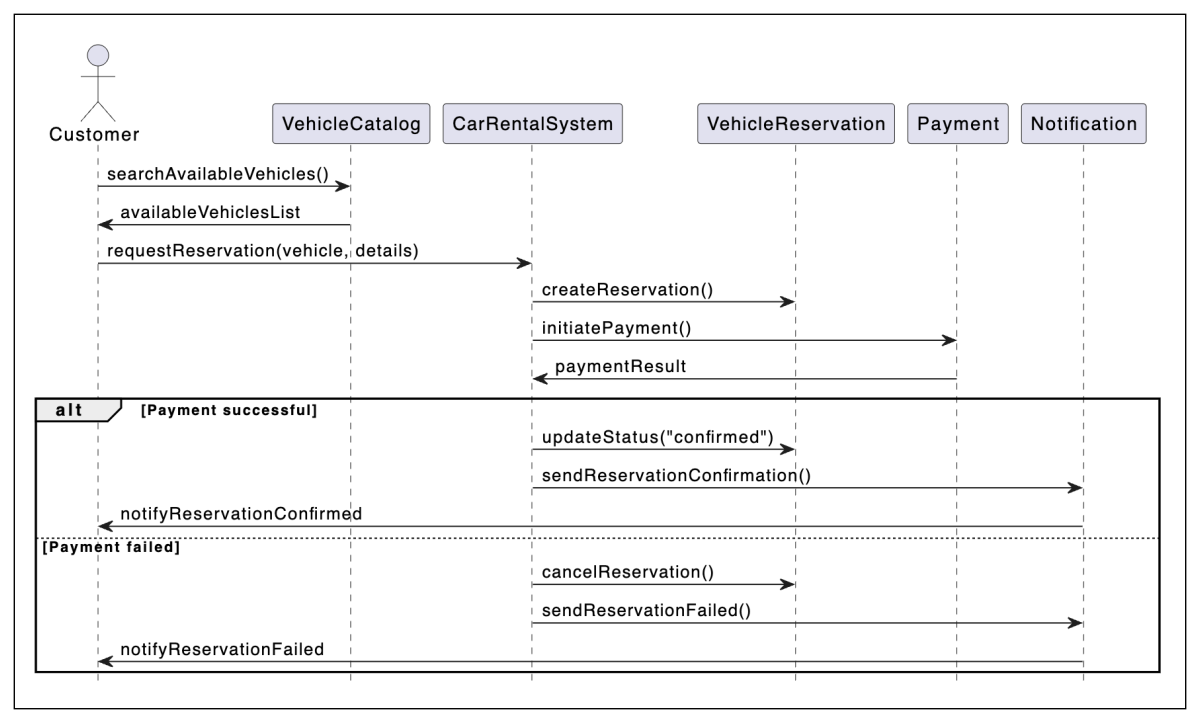
\includegraphics[width=0.5\textwidth]{Images/chapter_15/section_6250981438521344/5804445072752640.png}
 \caption{The sequence diagram for vehicle reservation}
\end{figure}

\subsection{Sequence challenge: Cancel reservation}\label{fHxT_dVYp6FmPOr1CFhnN}
\\
You'll help us complete a sequence diagram for a reservation canceled by the member. A skeleton of the cancel reservation sequence diagram is given below:

\begin{figure}[htbp]
 \centering
 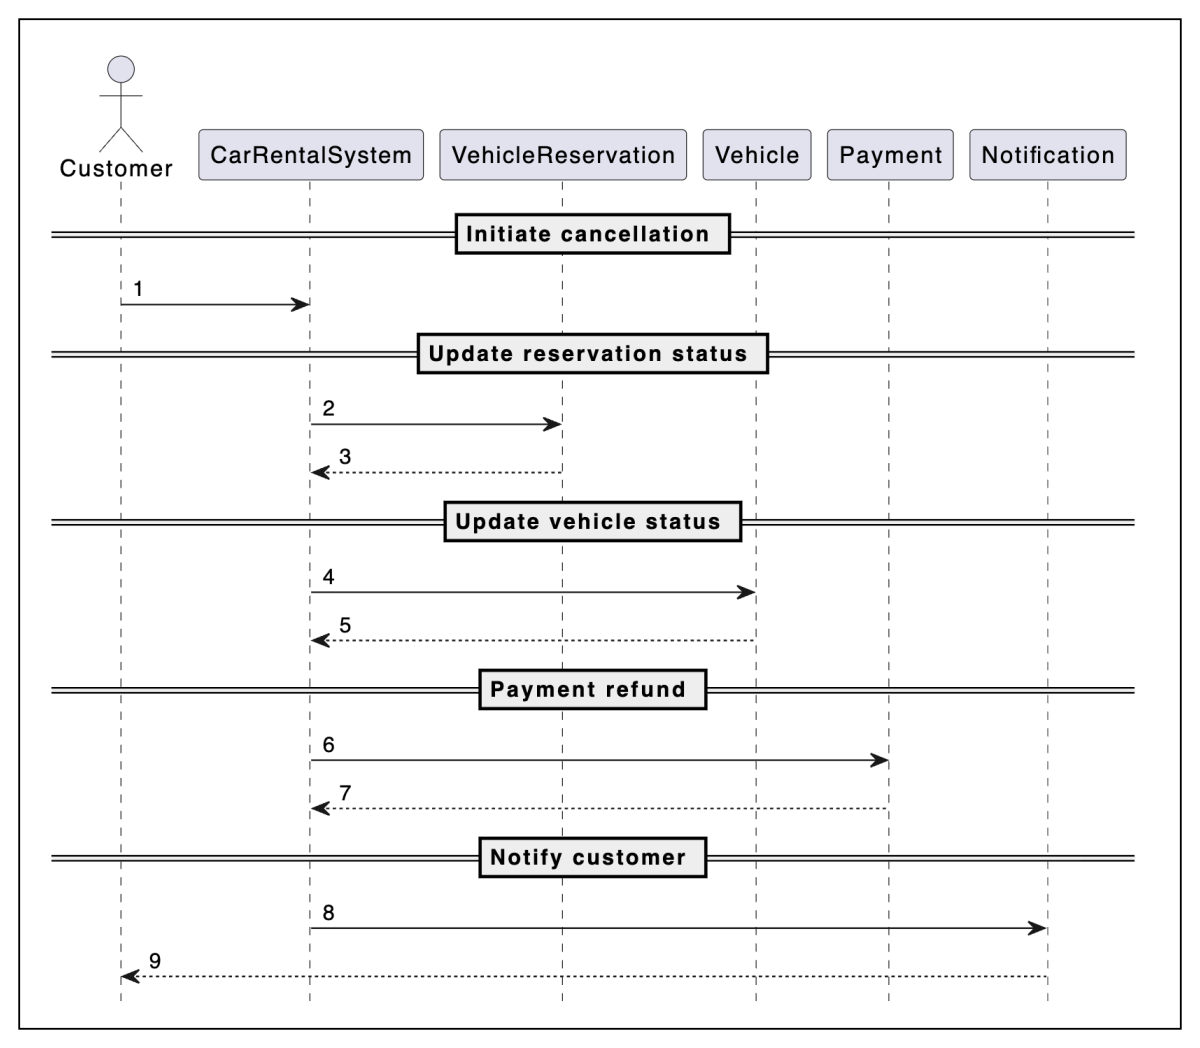
\includegraphics[width=0.5\textwidth]{Images/chapter_15/section_6250981438521344/4752228530126848.png}
 \caption{The sequence diagram for canceling a reservation}
\end{figure}

Notice that the arrows in the diagram above are numbered from 1 to 9. Below are the messages between the actor(s) and object(s). Can you rearrange the messages below in the correct sequence of order they should appear in the skeleton of the sequence diagram given above?
\begin{quote}
\textbf{Note:} If you're stuck, click the ``Show Solution'' button.
\end{quote}

Alternatively, you can also click the ``Show complete diagram'' button below to view the complete sequence diagram of the cancel reservation interaction.

\textless img src=``/udata/k8qEJqqnpYa/Car Rental.png'', width=700\textgreater{}

Next, let's examine the activity diagrams for the car rental system to understand its control flow.

% End of section content